%summary for PROG1

\documentclass[french]{article}
\usepackage[utf8]{inputenc}
\usepackage[T1]{fontenc}
\usepackage{babel}
\usepackage{lmodern}
\usepackage{graphicx}
\usepackage{tikz}
	\usetikzlibrary{arrows}

\usepackage{amsmath}
\usepackage{amsfonts}

\usepackage{float}

\title{Programmation 1}
\date{}
\author{L3 RI}


\begin{document}
\maketitle
\tableofcontents
\newpage

\section{CamL}

\subsection{Introduction à CamL}
Robin Milner (ML : meta-language).
Typer = démontrer.
P.L Curien crée CAM (categorical abstract machine)
$\Rightarrow$ CAML.

Inférence de type : résolution de l'équation aux domaines (résoudre une équation de types).

<fun> place-holder.

\subsection{CamL et orienté objet}
Liste : constructeurs, extracteurs, observateurs, combinateurs.

car (hd) : Content Adress Register.\\
cdr (tl) : Content Decrement Register.

API (Application Programming Interface) fait le lien entre concret et abstrait. Types abstraits $\mapsto$ module.

\subsection{Théorie des catégories}
Catégories : Set, Group, Ring, Field, Vector. $\neq$ ensemble (cf paradoxe B. Russell).

Objet terminal T : $A \rightarrow\up{$\exists$!}\ T$.

Objet initial I : $I \rightarrow\up{$\exists$!}\ A$.

Somme et produit : Unique à un iso. près.

%
\begin{table}[H]
	\centering
	\begin{tabular}{|c|c|}
		\hline
		Produit & Somme \\
		\hline
		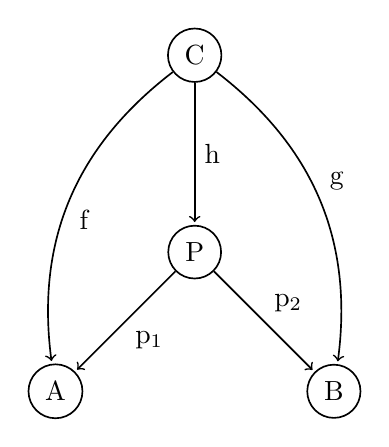
\begin{tikzpicture}[->, shorten >=1pt, auto, node distance=2.5cm, main node/.style={circle, draw}, semithick]
			\node[main node] (C) {C};
			\node[main node] (P) [below of=C] {P};
			\node[main node] (A) [below left of=P] {A};
			\node[main node] (B) [below right of=P] {B};
			
			\path
				(C) edge [bend right] node {f} (A)
				(C) edge [bend left] node {g} (B)
				(C) edge node {h} (P)
				(P) edge node {p$_1$} (A)
				(P) edge node {p$_2$} (B)
			;
		\end{tikzpicture}
		&
		\begin{tikzpicture}[->, shorten >=1pt, auto, node distance=2.5cm, main node/.style={circle, draw}, semithick]
			\node[main node] (C) {C};
			\node[main node] (S) [below of=C] {S};
			\node[main node] (A) [below left of=P] {A};
			\node[main node] (B) [below right of=P] {B};
			
			\path
				(A) edge [bend left] node {f} (C)
				(B) edge [bend right] node {g} (C)
				(S) edge node {h} (C)
				(A) edge node [bend left] {i$_1$} (S)
				(B) edge node [bend right] {i$_2$} (S)
			;
		\end{tikzpicture} \\
		\hline
	\end{tabular}
\end{table}
%

\subsection{Références}
Assigner un nom à une boîte, pas à une valeur. Modifier boîte $\rightarrow$ impureté, effet de bord.

Structures modifiables en CamL : type t = $\{$a : int ref$\}$.

\subsection{Les exceptions}
Changement de thread. Un déroutement peut être matériel, système (kernel panic) ou programme.

CamL : try TrucQuiPeutRaise with |telleException -> tel traitement.

\subsection{Programmation d'ordre supérieure}
Appeller une fonction avec ses paramètres et un futur : une fonction qui va s'appliquer au résultat. On peut alors prendre un futur excpetionnel ou faire du pipeline.

On peut empiler des fonctions dans le futur (ex factorielle).


\section{Scala - OOP et FP}

\subsection{OOP}

Classes, classes abstraites, constructeurs, champs, méthodes

Instances de classe

Héritage, composition, agrégation

\subsection{FP}

Fonctions, composition de fonctions

Pas de variables globales

Utilisation de "Pattern-matching"



\end{document} 

